\section{The \textit{Crude Petroleum and Natural Gas} Trade Network}

% - pl nel tempo
% - two strange pl plottati
% 	GAS 2006, in_degree + w
% 	FOOD 2010, in_degree + w
% - network plot
% - nodi fighi
% - ts delle metriche del nodo (pr, degree, weight degree, h/a)
% - plot communities chschshchs (sbm & louv) -> chose year
% - plot network (sbm & louv)

%     1) graph metrics:
%         - over time
%         - power law over time
%     2) node properties:
%         - compared on average tra i nodi
%         - time series of relevant node's + pr
%     3) communities:
%         - grafico schschschschscsch (x2)
%         - plot confronto sbm vs louv 
%             --> fai vedere in cosa sono diversi (perchè le communities rappresentano cose diverse)
%             --> confronto modularities
%         - plot tanti^n plot

The second category that I am going to investigate is \textit{Crude Petroleum and Natural Gas}\footnote{
    From the EU Economic Activity Classification:
    "This division includes the production of crude petroleum, the mining and extraction of oil from oil shale and oil sands and the production of natural gas and recovery of hydrocarbon liquids. This division includes the activities of operating and/or developing oil and gas field properties. Such activities may include drilling, completing and equipping wells; operating separators, emulsion breakers, desalting equipment and field gathering lines for crude petroleum; and all other activities in the preparation of oil and gas up to the point of shipment from the producing property."\cite{eurostat2022website}
}. 
The trade market of Oil and Gas is an essential pillar of international trade, which in 2019 moved around more than XXXX million euros worth of exports. It is the nature of the good itself which makes it a suitable item to be exchanged. In fact, only relatively few countries in the world have access to underground fossil fuel resources, and even less countries have enough of it to be great exporters on the global landscape. According to COMEXT-WTO data, the XXX\% of total global exports of \textit{Crude Petroleum and Natural Gas} were coming from just Y different countries: A,B,C,D,E.
This fact is an indicator of the presence of an oligopoly\footnote{
    An \textit{oligopoly} is a market structure in which a market or industry is dominated by a small number of large sellers or producers. Oligopolies often result from the desire to maximize profits, leading to collusion between companies. This reduces competition, leading to higher prices for consumers and lower wages for employee (from \url{https://en.wikipedia.org/wiki/Oligopoly}).
}, which is a renowned fact in microeconomic research, so that very often it is used as an example of these types of markets \cite{mileva2012oil}.
An oligopolistic structure, however, together with the fact that oil and gas are essential goods for the majority of industrialized modern countries, has the potential to create instability into these countries, should any event disrupt or prevent the full functioning of the trade exchanges. An example of a disruption that had an impact on the global supply chain was the Suez Canal blockage of March 2021 \cite{lee2021suez}, while a more recent event of greater magnitude for the global stability is the Russian invasion of Ukraine of 2022. Earlier this year, on February 24th, Russia crossed the border with Ukraine with military forces: this situation is the result of a long deterioration of the relationships among the two nations and a lengthy streak of violence. It started in 2014 with the Ukrainian revolution and the subsequent detachment of the country from the orbit of pro-Russian nations to institute a pro-western government.
The return of war at the heart of the European continent provoked a shock in the neighboring countries which has had few equals in the history of the community; numerous helps of varying nature have been offered to Ukraine, including financial, humanitarian and also military aid. For this research, the most important aspect is certainly the one concerning the economic sanctions imposed on Russia. In fact, one of the sectors that most drives the Russian economy is that of import-export, especially of natural gas and raw materials to various European countries such as Italy, the Czech Republic and Austria. If, on the one hand, the European Union, considering the close dependence of various countries internally, has imposed significant sanctions on oil, but not on natural gas, on the other hand Russia itself has made several cuts in supplies and raised the prices of this scarce but essential resource \cite{sole2022petrolio,wikipedia2022crisirussia}.
% https://www.ilsole24ore.com/art/petrolio-oro-gas-che-punto-sono-sanzioni-ue-russia-AEyWcbiB
% https://it.wikipedia.org/wiki/Crisi_russo-ucraina
% Il 24 febbraio 2022 la Russia invade l'Ucraina. Questa situazione è stata il risultato di un lungo deterioramento dei rapporti tra i due stati e una lunga successione di violenze, cominciata nel 2014 con la rivoluzione Ucraina e il conseguente distaccamento di quest'ultima dall'orbita degli stati filo-russi per instaurare, invece, un governo filo-occidentale.
% Il ritorno della guerra nel cuore dell'Europa ha provocato uno shock da parte delle altre nazioni che ha avuto pochi eguali nella storia comunitaria; sono stati forniti aiuti di varia natura all'Ucraina, sia dal punto di vista economico, sia dal punto di vista umanitario. Per questo studio, l'aspetto più importante è sicuramente quello che riguarda le sanzioni economiche imposte alla Russia. Infatti, uno dei settori che maggiormente traina l'economia russa è quello dell'import-export, soprattutto di materie prime ai vari paesi Europei come Italia, Repubblica Ceca e Austria.
% Se l'Unione Europea, considerando la stretta dipendenza di vari paesi al proprio interno, ha imposto sanzioni significative sul petrolio, ma non sul gas naturale. La stessa Russia, invece, ha effettuato diversi tagli alle forniture e ha alzato i prezzi di questa risorsa così scarsa ma così essenziale.
Thanks to the availability of data and the tools of network science, we can try to find a reason for why a disruption such as Russia cutting off its gas supply could have such a shaking effect on Europe and the limiting countries. I will follow the same steps as the previous analysis, and thus I will start by having a look at the aggregated metrics of the graph over time. 
In Figure \ref{fig:gasmetrics} we see the time series of the network's \textit{size}, average \textit{degree}, median \textit{page rank} and average \textit{clustering coefficient}. Looking at the upper left plot, we immediately see the effect of the two crises on the trade network size. In the 2008 financial crisis, the amount of trade dropped by more than 10 million euros (per 1000 p.) from one year to the next, while for COVID it even halved in 2020 with respect to 2019. A similar effect can be found in the average degree plot, with the 2020 crisis causing a sudden drop in the mean number of connection of nodes, due to many of these exchanges coming to a halt. Being this market an oligopoly, we may be expecting a higher page rank since a lot of nodes receive incoming edges without having any outgoing, but this is justified by the fact that the exporter nodes which would pass on the page rank to them have a lot of out going links, and thus each of them receives only a small portion of it.

\begin{figure}
    \centering
    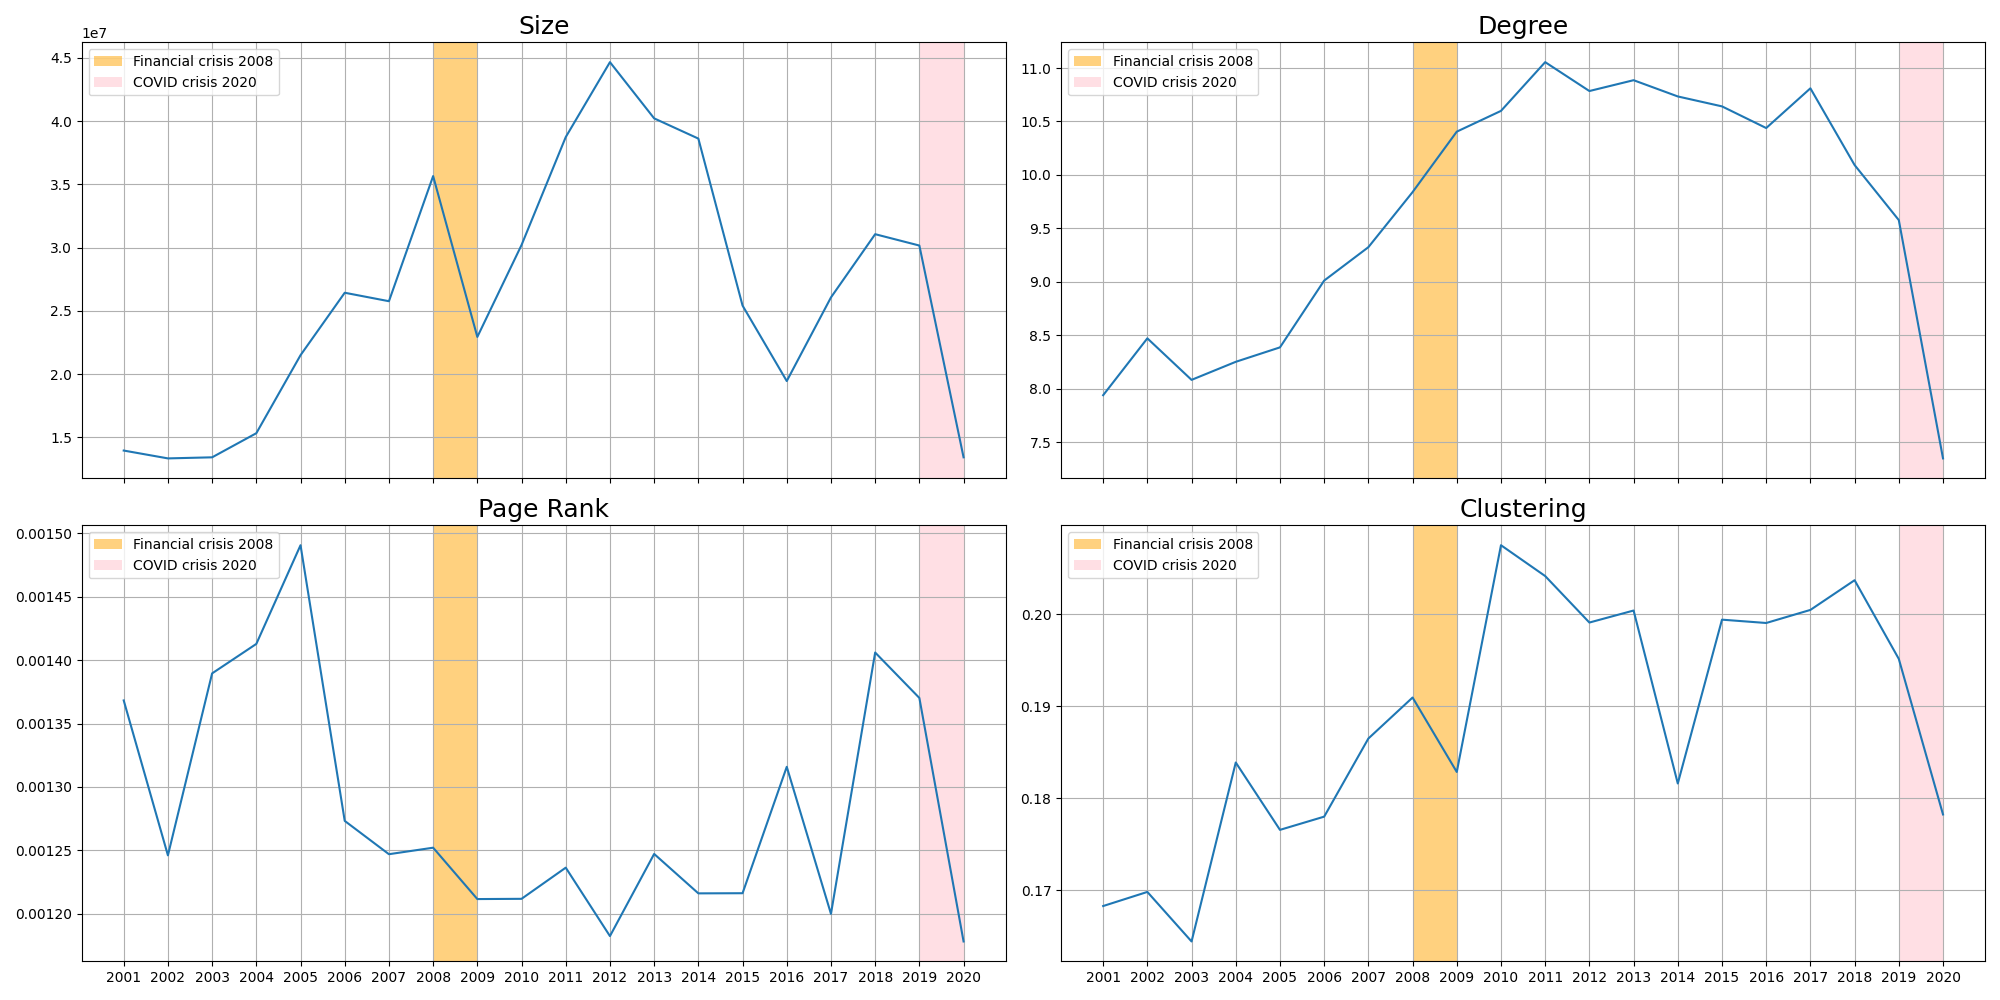
\includegraphics[width=\textwidth]{pics/full_p06_metric_ts.png}
    \caption{Crude petroleum and natural gas Metrics TODO}
    \label{fig:gasmetrics}
\end{figure}

\subsection{Degree distribution}

A secondary query we might try to find an answer to is whether in this trade sector the networks display signs of the \textit{scale-free} property. Hence, we look at Figure \ref{fig:gasdegree}, representing the power law fit over time. Considering the orange lines, indicating the fit of the linear regression in the log-log plot of the degree distribution, which is measured with MAPE, we see that the two weighted metrics are consistently a better fit than the unweighted version. Regarding the values of the \textit{gamma} exponent of the power law, it is similar in all four distributions, oscillating between the values of $0.8$ and $1$. Let us have a look at a specific year, to see whether it is indeed the case of a good power law fit.

\begin{figure}
    \centering
    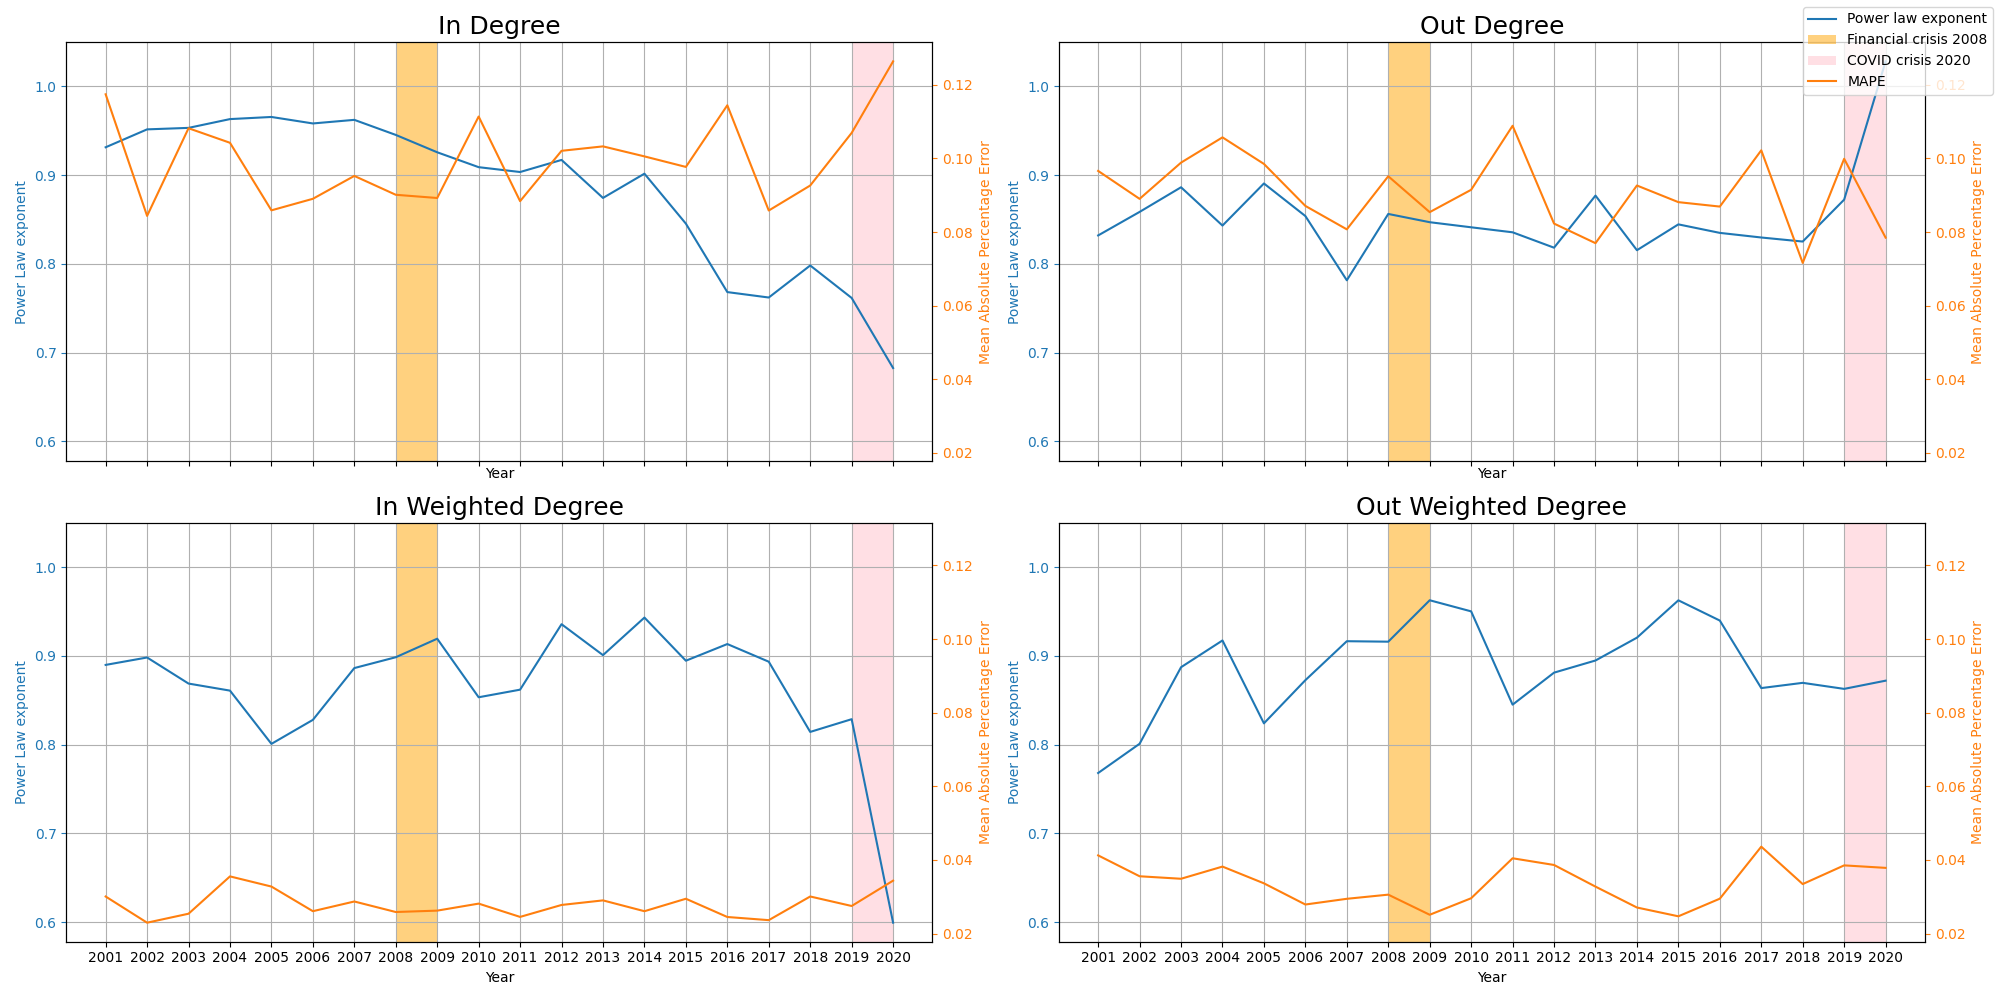
\includegraphics[width=\textwidth]{pics/ts_p06.png}
    \caption{Power law exponents over time of four degree distributions in the \textit{Crude petroleum and natural gas} networks.}
    \label{fig:gasdegree}
\end{figure}

Figure \ref{fig:gasdistrib} displays the degree distribution of the \textit{out degree} and \textit{out weighted degree} of the petroleum and gas trade network in 2010. Both curves seem to be quite fit to the distributions, and in particular the second one, which in fact presents a lower MAPE. The way we can interpret these plots is that the countries which have a high \textit{out degree} are the few oligopolistic exporters of the trade network, while the numerous countries with low degree are those who import from them. The \textit{out weighted degree} distribution is even more unbalanced than the previous one, with very few nodes which have an enormous output of gas and petroleum with respect to a great number of nodes which have no ability to export. By looking even more carefully at the dataset number, we can discover that the isolated point to the bottom right of the plot of the out weight degree is Russia alone, which has in fact a total export normalized value which is three times higher than the second major exporter, Saudi Arabia (although in nominal value they export roughly the same, Russia is known to sell petroleum and gas at a considerably lower price than other countries, thus the output quantity of RU corresponding to that monetary value is huge) \cite{trent2020opec}.
Let us have a look now in the next paragraph at the network plot for the trade of \textit{Crude petroleum and natural gas} in 2010.
% - both quite fit, the second better 
%     1 --- > the countries with high degree are the few exporters
%     2 --- > symptom of small number of countries which are completely dependent on gas from others

\begin{figure}
    \centering
    \begin{subfigure}{\textwidth}
        \centering
        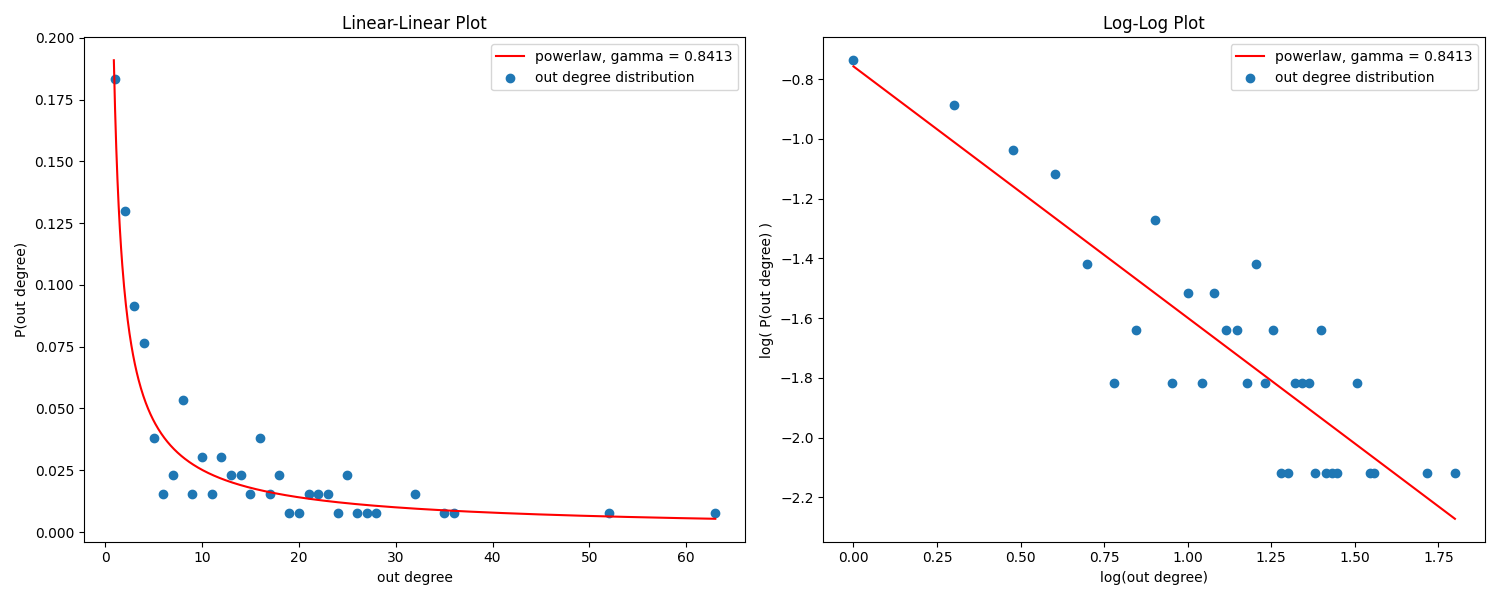
\includegraphics[width=\textwidth]{pics/powerlaw_out_degree_p06_y2010.png}
        \caption{\textit{Out Degree}}
        \label{fig:plgas}
    \end{subfigure}
    
    \begin{subfigure}{\textwidth}
        \centering
        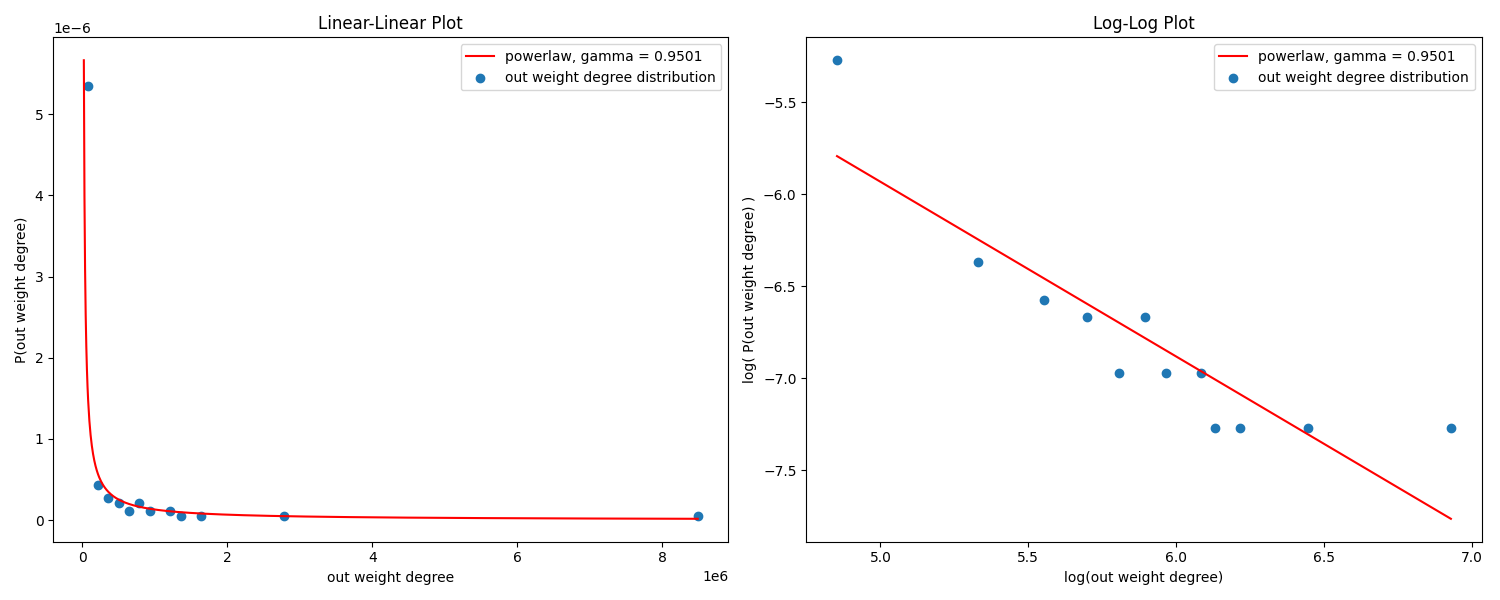
\includegraphics[width=\textwidth]{pics/powerlaw_out_weight_degree_p06_y2010.png}
        \caption{\textit{Out Weighted Degree}}
        \label{fig:plgasw}
    \end{subfigure}
    \caption{\textit{Crude petroleum and natural gas} trade network's degree distribution in 2010, with power law fit.}
    \label{fig:gasdistrib}
\end{figure}


\subsection{Network plot and node properties}

The plot in Figure \ref{fig:gasnetwork} of the petroleum and gas network is represented with the force-directed layout, which permits us to comment on the position of countries in the network. Indeed, we find positioned in the middle of the graph, countries which are the major global players in this market, and they are linked through a dense web of exchanges with other countries: they are Russia (RU), Saudi Arabia (SA), Arab Emirates (AE), Qatar (QA) and Norway (NO). The size of the node itself indicates the total output, and as it was mentioned above, Russia is by far the biggest in terms of normalized output. From there, a lot of thick edges (indicating heavier links) origin and go towards EU countries (\textit{pink} edges) or non-EU (\textit{azure} edges). A notable difference with the network of \textit{Food Products} is that in this case, many EU countries (indicated in \textit{blue}) become peripheral countries, which only receive imports of gas and don't produce any for export. There are a few EU countries in the middle which often act as redistributors, such as the Netherlands (NL), France (FR) and the United Kingdom (GB): they receive imports from other central countries and then export part of it to their neighboring ones. An additional characteristic that we can notice in the plot is a thick web of azure exchanges in the lower part of the network, surrounding the countries of SA, QA, AE. This represents the trade of petroleum and gas which originates from Middle East countries, and the receiving ends of those edges are countries which depend on such producers: in particular, among the highest importers of these good there are the United States (US), Japan (JP) and China (CN), all of which have an \textit{in degree} of more than 30 (in the case of China it is 53, which the highest among world countries).


\begin{figure}
    \centering
    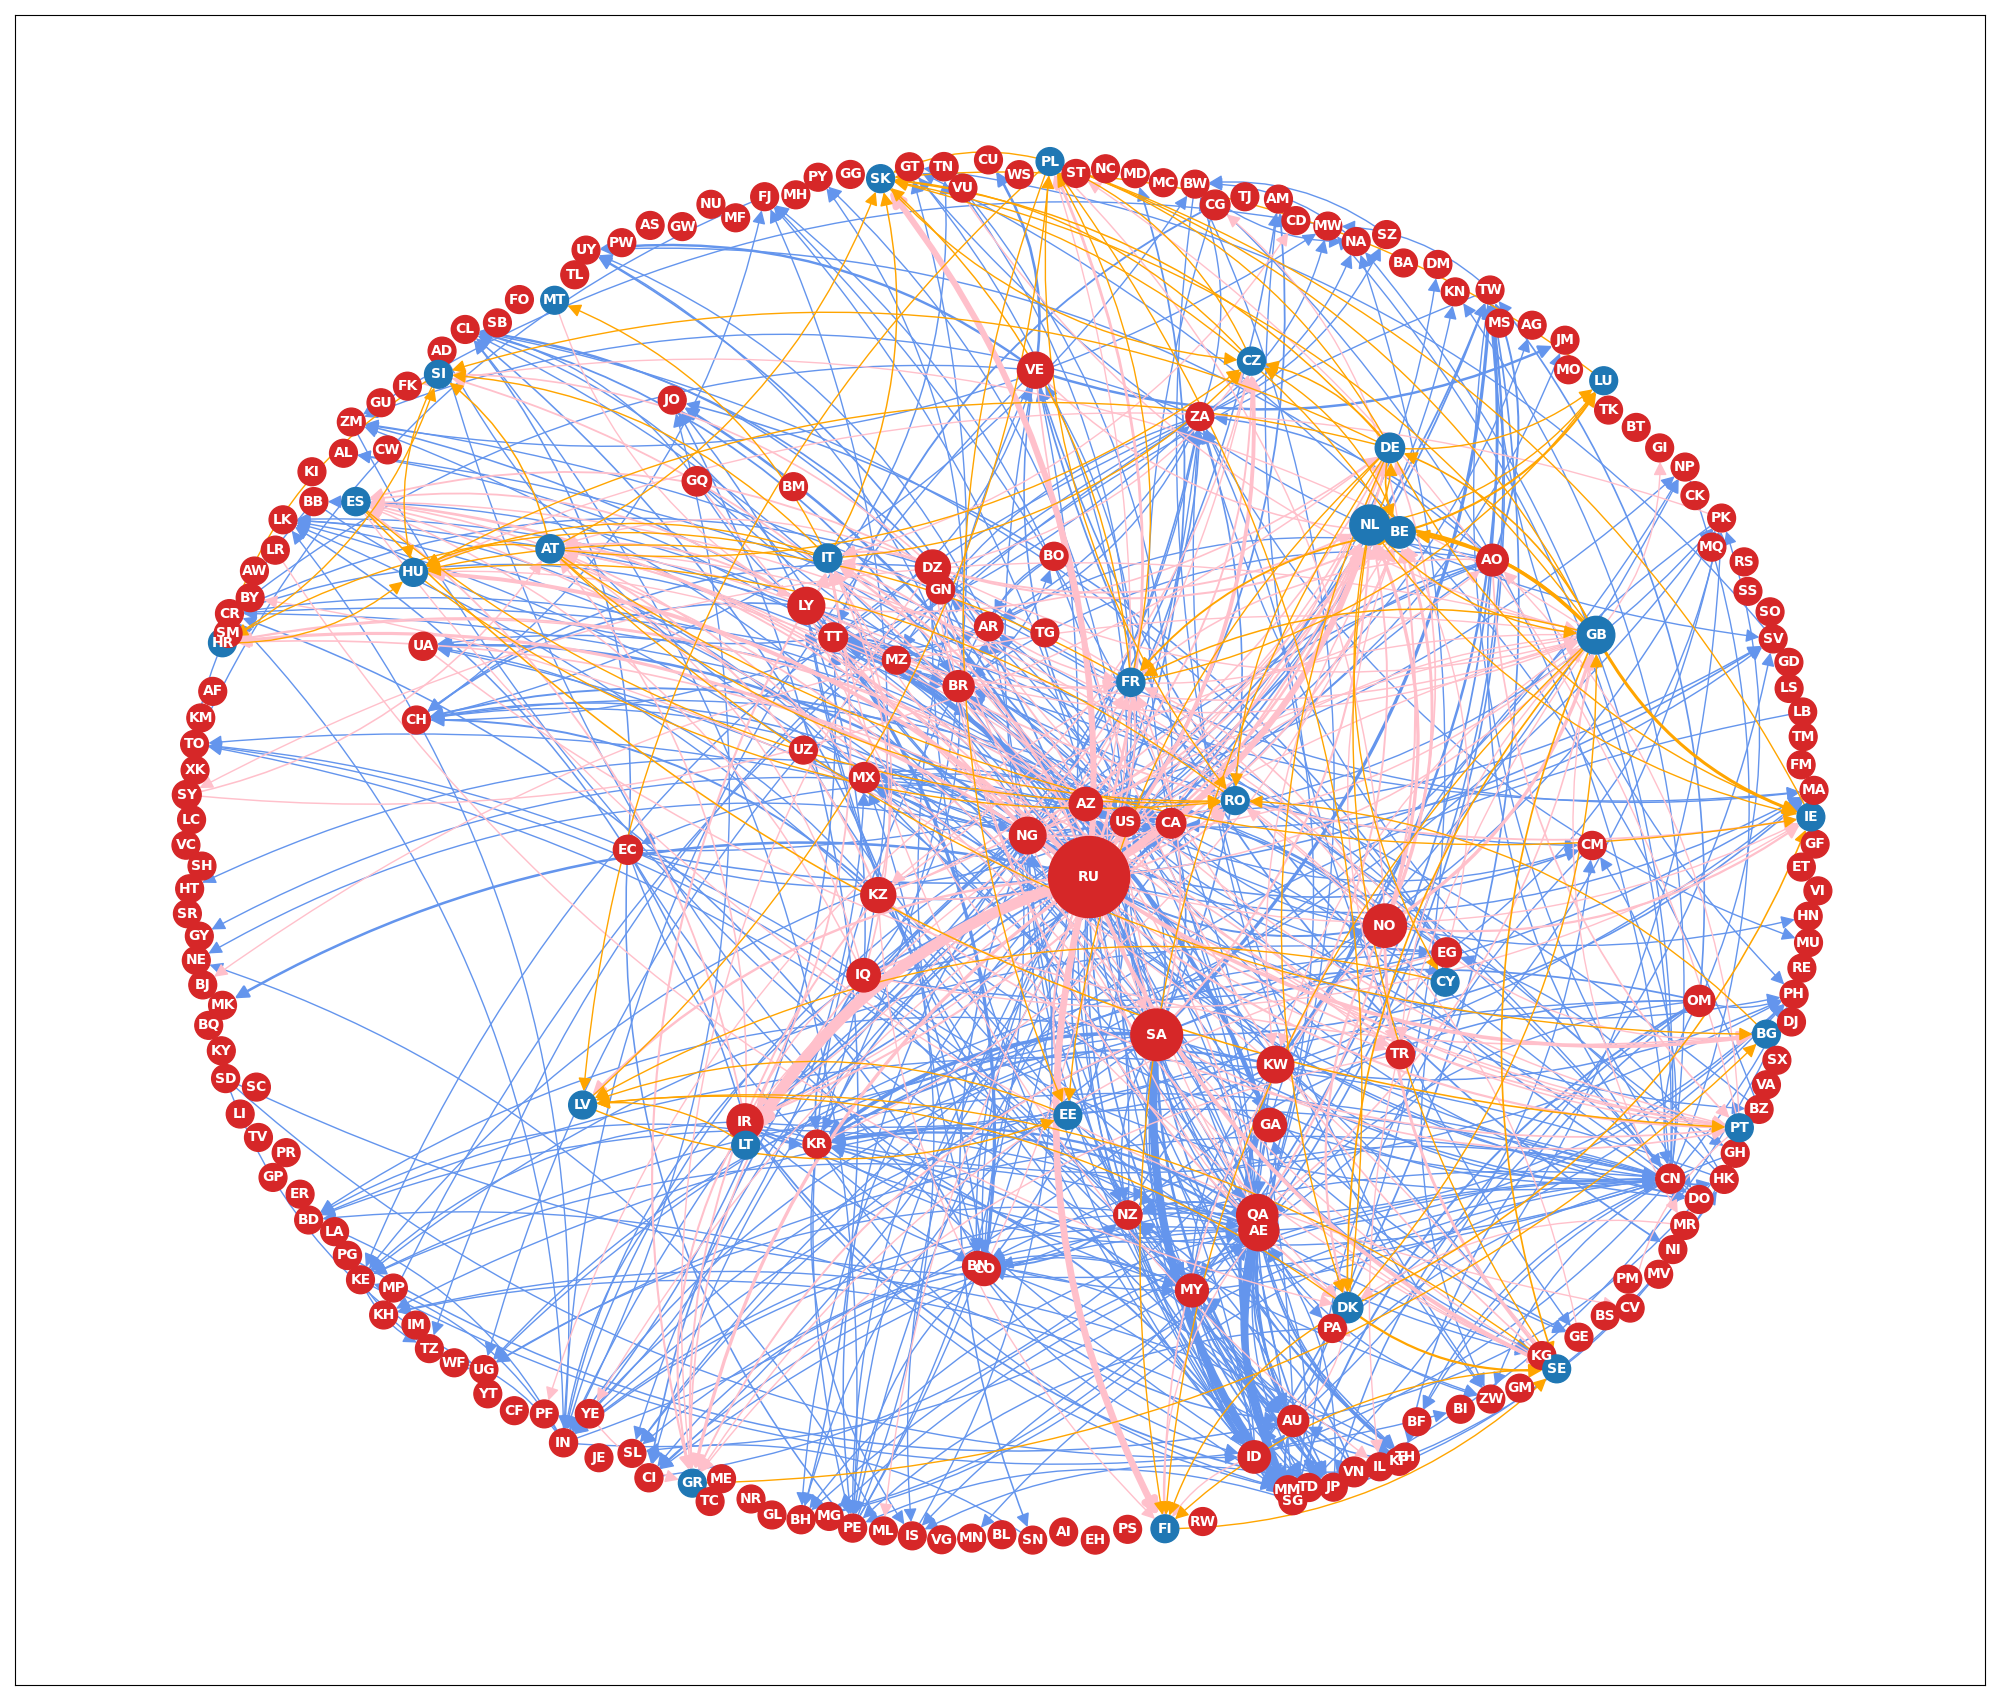
\includegraphics[width=\textwidth]{pics/full_y10_p06_force_120.png}
    \caption[Global trade network of \textit{Crude petroleum and natural gas} in 2010.]{Global trade network of \textit{Crude petroleum and natural gas} in 2010. The size of the node represents the \textit{out-strength} of that country. The color of the node indicates EU countries (\textit{blue}) and non-EU (\textit{red}); the color of the edge is \textit{orange} for intra-EU exchanges, \textit{pink} for EU - non-EU exchanges and \textit{azure} for extra-EU exchanges. Only the top 5 import partnership for each country are shown.}
    \label{fig:gasnetwork}
\end{figure}

Nevertheless, the high count of import partnerships of these countries is a valuable strategy in assuring continuous supply of this good, and in fact they don't appear on the top list of highest dependencies on petroleum and gas supplies, neither in 2010, nor more recently in 2019 (which is shown in \cref{tab:top10gasimp}). The numbers in this table provide evidence in support of the claim that countries, especially European ones, depend on Russian imports. Five out of ten exports of this table are links from Russia to countries such as Lithuania (LT), Finland (FI) and the Netherlands (NL), and we see that the situation has remained stable also in 2019. 
For what it concerns Italy, instead, we observe a change in behavior over the course of nine years. Figuring at the top of imports of \textit{Crude petroleum and natural gas} in 2010 there were Libya (LY), Russia (RU) and Algeria (DZ), at around similar levels. The situation has changed in 2019, where only Russia has maintained its status as leading supplier for Italy, whereas Libya and Algeria basically halved their exports in terms of normalized values. A possible cause of this may have been the Libyan crisis of 2011, linked with the riots and protests across all Middle Eastern and North African countries, known as the "Arab Spring" \cite{wikipedia2011libia}.

\begin{table}
    \centering
    % \resizebox{0.45\textwidth}{!}{
    \resizebox{0.3\textwidth}{!}{
\begin{subtable}{0.3\textwidth}
    \centering
    \begin{tabular}{llr}
    \toprule
    Country From & Country To & Value €/1000 p. \\
    \midrule
              RU &         LT &      1559671.18 \\
              NL &         BE &      1182214.94 \\
              SA &         SG &      1072159.63 \\
              RU &         FI &       862697.08 \\
              RU &         NL &       794297.04 \\
              QA &         SG &       760397.50 \\
              RU &         SK &       757951.78 \\
              AE &         SG &       578737.40 \\
              GA &         TT &       447159.96 \\
              RU &         SE &       415147.96 \\
    \midrule
              LY &         IT &       179972.18 \\
              RU &         IT &       163684.12 \\
              DZ &         IT &       124351.88 \\
              AZ &         IT &        88476.04 \\
              IR &         IT &        73648.57 \\
              IQ &         IT &        52013.73 \\
              SA &         IT &        40190.73 \\
              KZ &         IT &        34114.82 \\
              QA &         IT &        24683.36 \\
              NO &         IT &        20077.77 \\
    \bottomrule
    \end{tabular}
    \caption{Year 2010}
    \label{tab:top10gasimport2010}
\end{subtable}
}
\hfill
\resizebox{0.3\textwidth}{!}{
\begin{subtable}{0.3\textwidth}
    \centering
    \begin{tabular}{llr}
    \toprule
    Country From & Country To & Value €/1000 p. \\
    \midrule
              NL &         BE &      1137264.82 \\
              RU &         LT &      1132888.14 \\
              AE &         SG &      1008058.09 \\
              GB &         GI &       975584.21 \\
              RU &         FI &       822037.96 \\
              QA &         SG &       678777.87 \\
              RU &         NL &       659501.86 \\
              RU &         SK &       496666.08 \\
              SA &         SG &       449912.07 \\
              ID &         SG &       438746.74 \\
    \midrule
              RU &         IT &       160747.70 \\
              AZ &         IT &        80488.00 \\
              IQ &         IT &        79245.86 \\
              LY &         IT &        73654.21 \\
              DZ &         IT &        60418.95 \\
              SA &         IT &        34539.17 \\
              KZ &         IT &        30295.88 \\
              NG &         IT &        23981.59 \\
              QA &         IT &        19787.63 \\
              US &         IT &        13775.67 \\
    \bottomrule
    \end{tabular}
    \caption{Year 2019}
    \label{tab:top10gasimport2019}
\end{subtable}
}
    % }
    \caption{Top 10 edges by weight in the \textit{Crude petroleum and natural gas} market and top 10 incoming edges for IT by weight, in 2019.}
    \label{tab:top10gasimp}
\end{table}

Given the central role that has Russia in this particular market, let us have a look at the single node's metrics and how they evolved in time, which might give us insights into the role of Russia in this trade market over the last 20 years. In \cref{fig:rusmetrics}, there are displayed six relevant metrics for the node centrality. It is interesting to see that the values of Page Rank and Authority are essentially constant at zero: this is not surprising since the role of Russia as one of the biggest world exporters implies that it has many edges which point towards other nodes, thus distributing the page rank. At the same time, there are basically no incoming edges for Russia, and this explains the Authority Value. On the contrary, having a high number of outgoing edges is what drives up the Hub value of RU. According to these plots, we could say that Russia had a peak of importance in the market in the three years of 2010-2012, as it can be derived from the high values of Hub, Out Degree and Out Weighted Degree. This is in line with the reported news that one can find on that period \cite{reutersru1,reutersru2}.

\begin{figure}
    \centering
    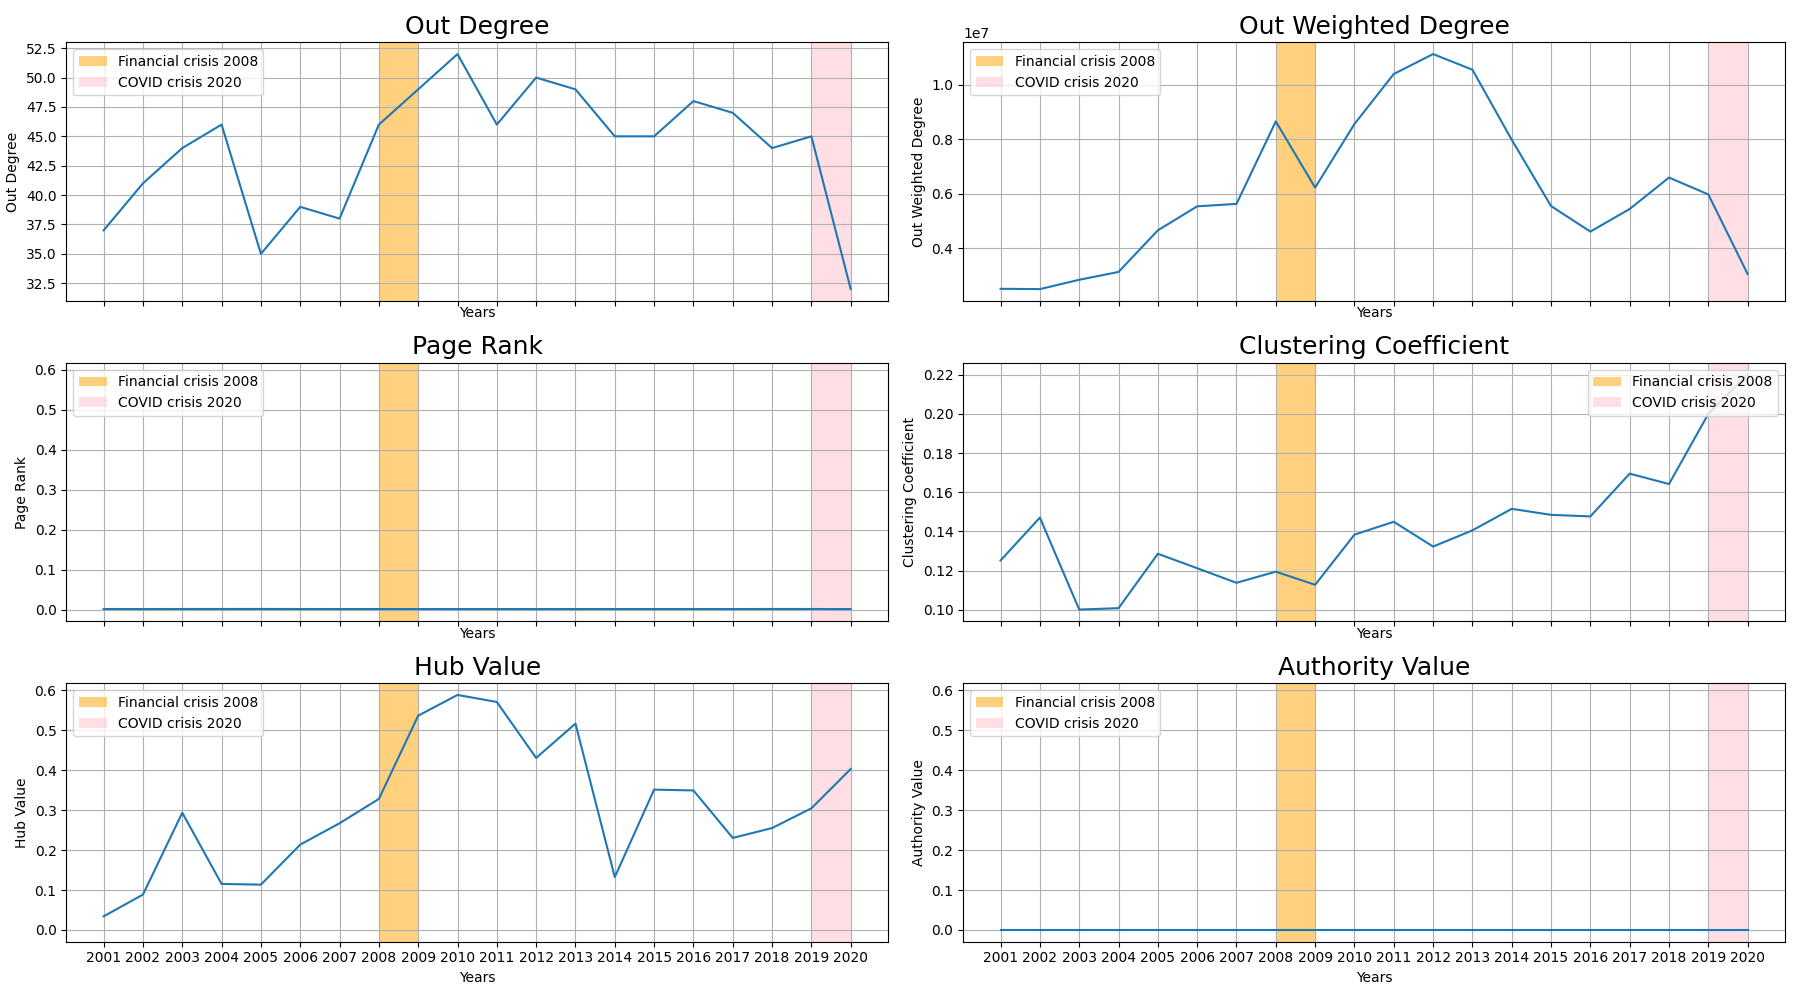
\includegraphics[width=\textwidth]{pics/RU_p06_metric_ts.png}
    \caption{Network metrics for Russia (RU) of the trade market of \textit{Crude petroleum and natural gas} over the years.}
    \label{fig:rusmetrics}
\end{figure}


\subsection{Community detection}

As it was done for the previous category, we can explore the outcomes of the algorithms for community detection (DCSBM and Louvain), in order to search for clusters of countries trading intensely or to see whether these present evidences of a core-periphery structure. Let us start by looking at the parallel categories plot of \cref{fig:commgas}. In this market sector, the Degree Corrected SBM has identified three communities in 2019 (\cref{fig:dcgas}), one of which, the yellow one (3), seems to have been defined since the first years. At the same time, also the output of the Louvain method (\cref{fig:lougas}) in 2019 is composed of three main communities, with two small additional ones. Given this results, it is of interest to understand whether the two algorithms have returned similar block memberships, that is to say whether the communities refer to the same set of nodes. The communities are plotted in \cref{fig:gascommunities}, once for each method. If we consider the first figure, we start by noticing that Russia (RU) has a different color than the Middle Eastern competitor countries, which instead belong to the green community. Therefore, we can conclude that the cluster of countries in purple (1) is made of those countries which have strong import partnerships with Russia (including Italy), while the cluster in green (2) comprises nodes which trade considerably with Saudi Arabia (SA), Arab Emirates (AE), Qatar (QA) and others. A similar community structure can be found in the second plot, from the Louvain method: here the cluster of nodes orbiting Russia is in green (3), while the Middle Eastern block is in blue (2). However, a relevant difference with DCSBM that we can observe here is the following: while in the previous plot the third community includes those nodes which are at the periphery of the network and don't have a relevant role in this trade market, in the second plot we see the third community at the center of the network, made of nodes such as the United States (US), Norway (NO), Canada (CA), the Netherlands (NL) and the United Kingdom (GB).

\begin{figure}
    \centering
    \begin{subfigure}{\textwidth}
        \centering
        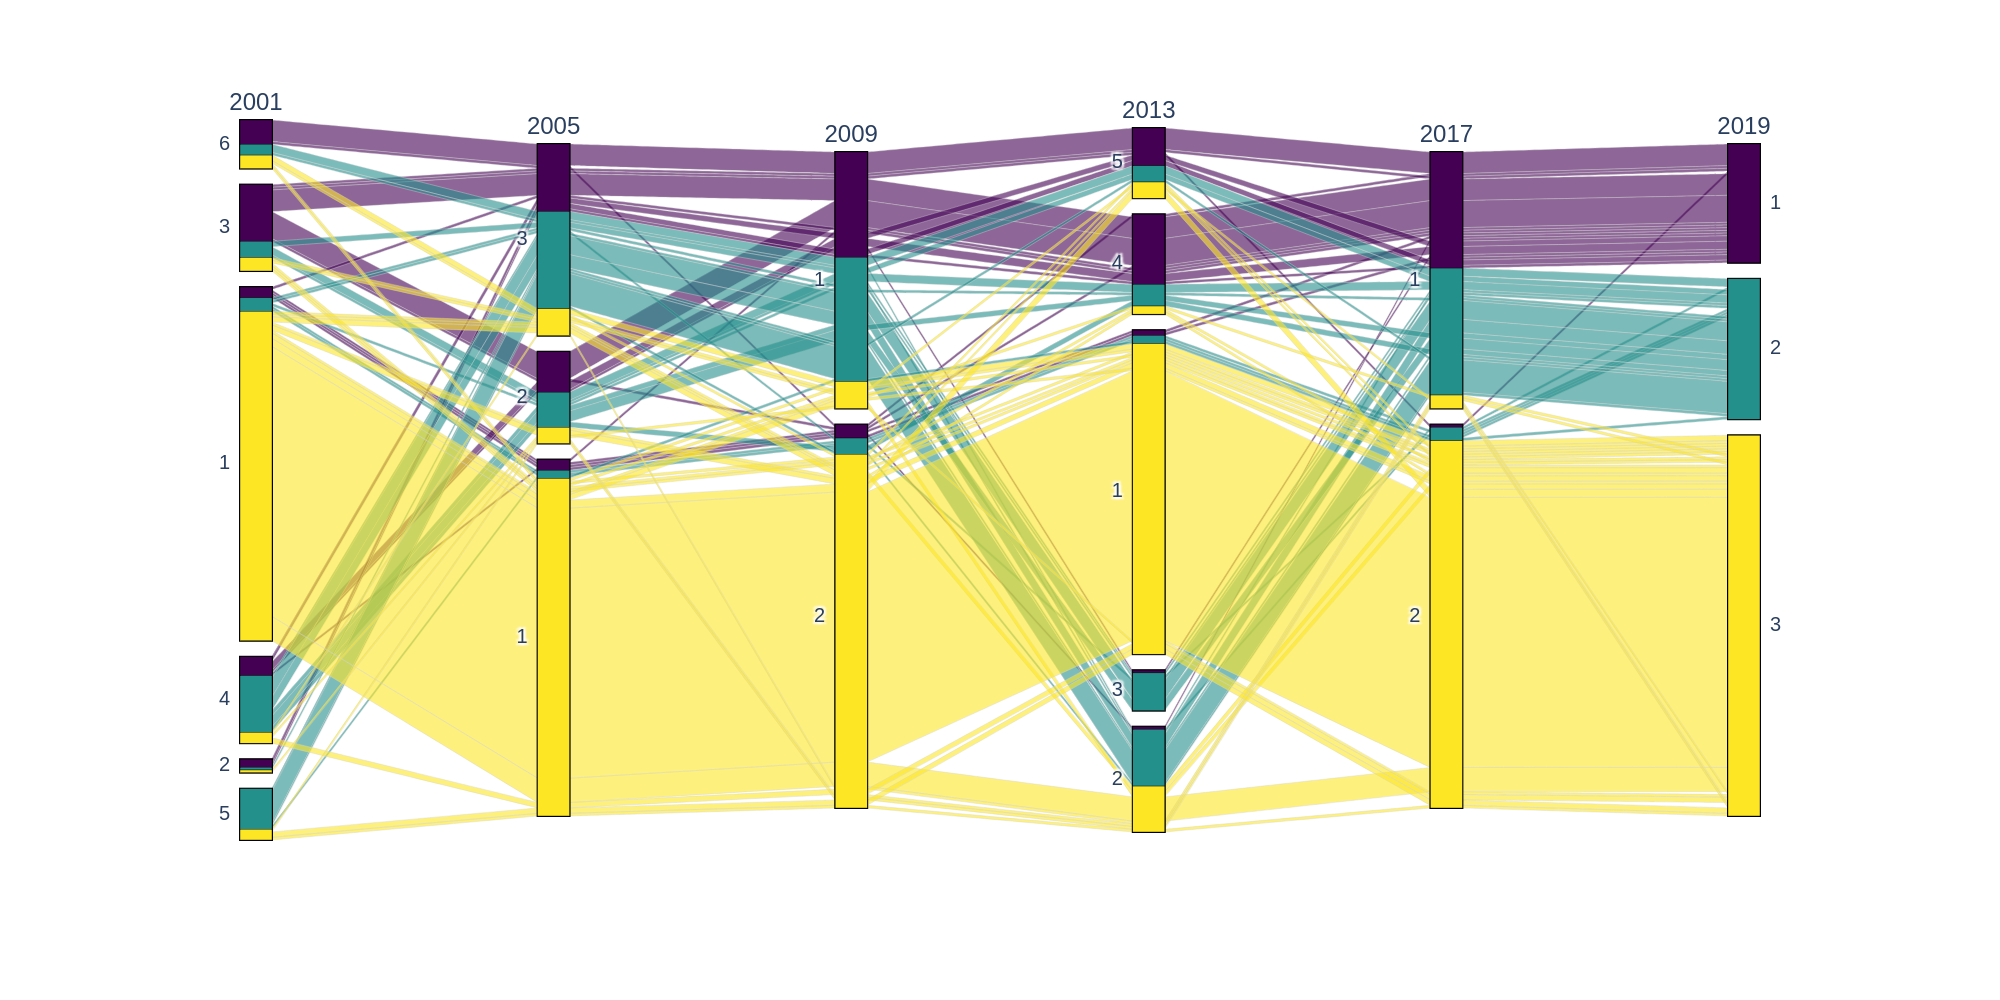
\includegraphics[width=\textwidth]{pics/dc_p06.png}
        \caption{Degree Corrected SBM}
        \label{fig:dcgas}
    \end{subfigure}
    \begin{subfigure}{\textwidth}
        \centering
        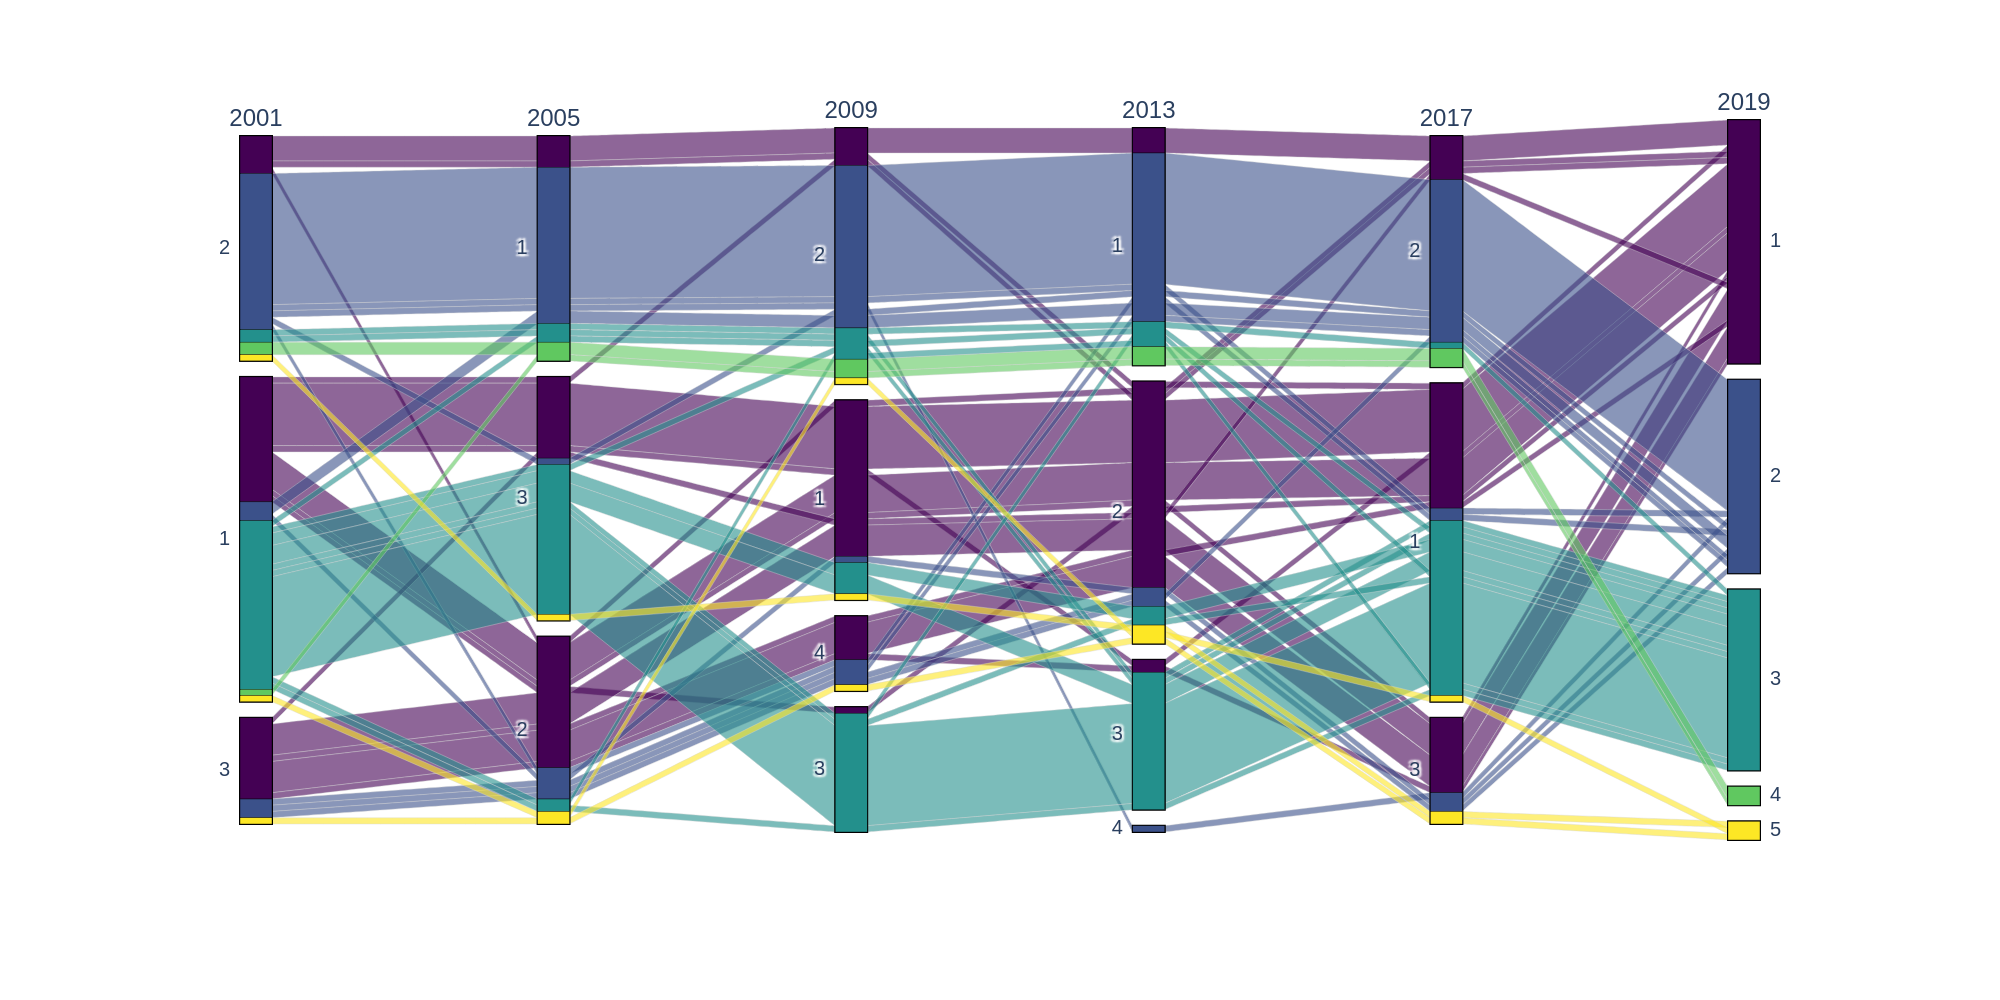
\includegraphics[width=\textwidth]{pics/lou_p06.png}
        \caption{Louvain Method}
        \label{fig:lougas}
    \end{subfigure}
    \caption[Evolution over time of the communities of the \textit{Crude petroleum and natural gas} trade network.]{Evolution over time of the communities of the \textit{Crude petroleum and natural gas} trade network. Communities are shown every 4 years, plus 2019. The colors refer to the memberships in 2019.}
    \label{fig:commgas}
\end{figure}


\begin{figure}
    \centering
    \begin{subfigure}{0.5\textheight}
        \centering
        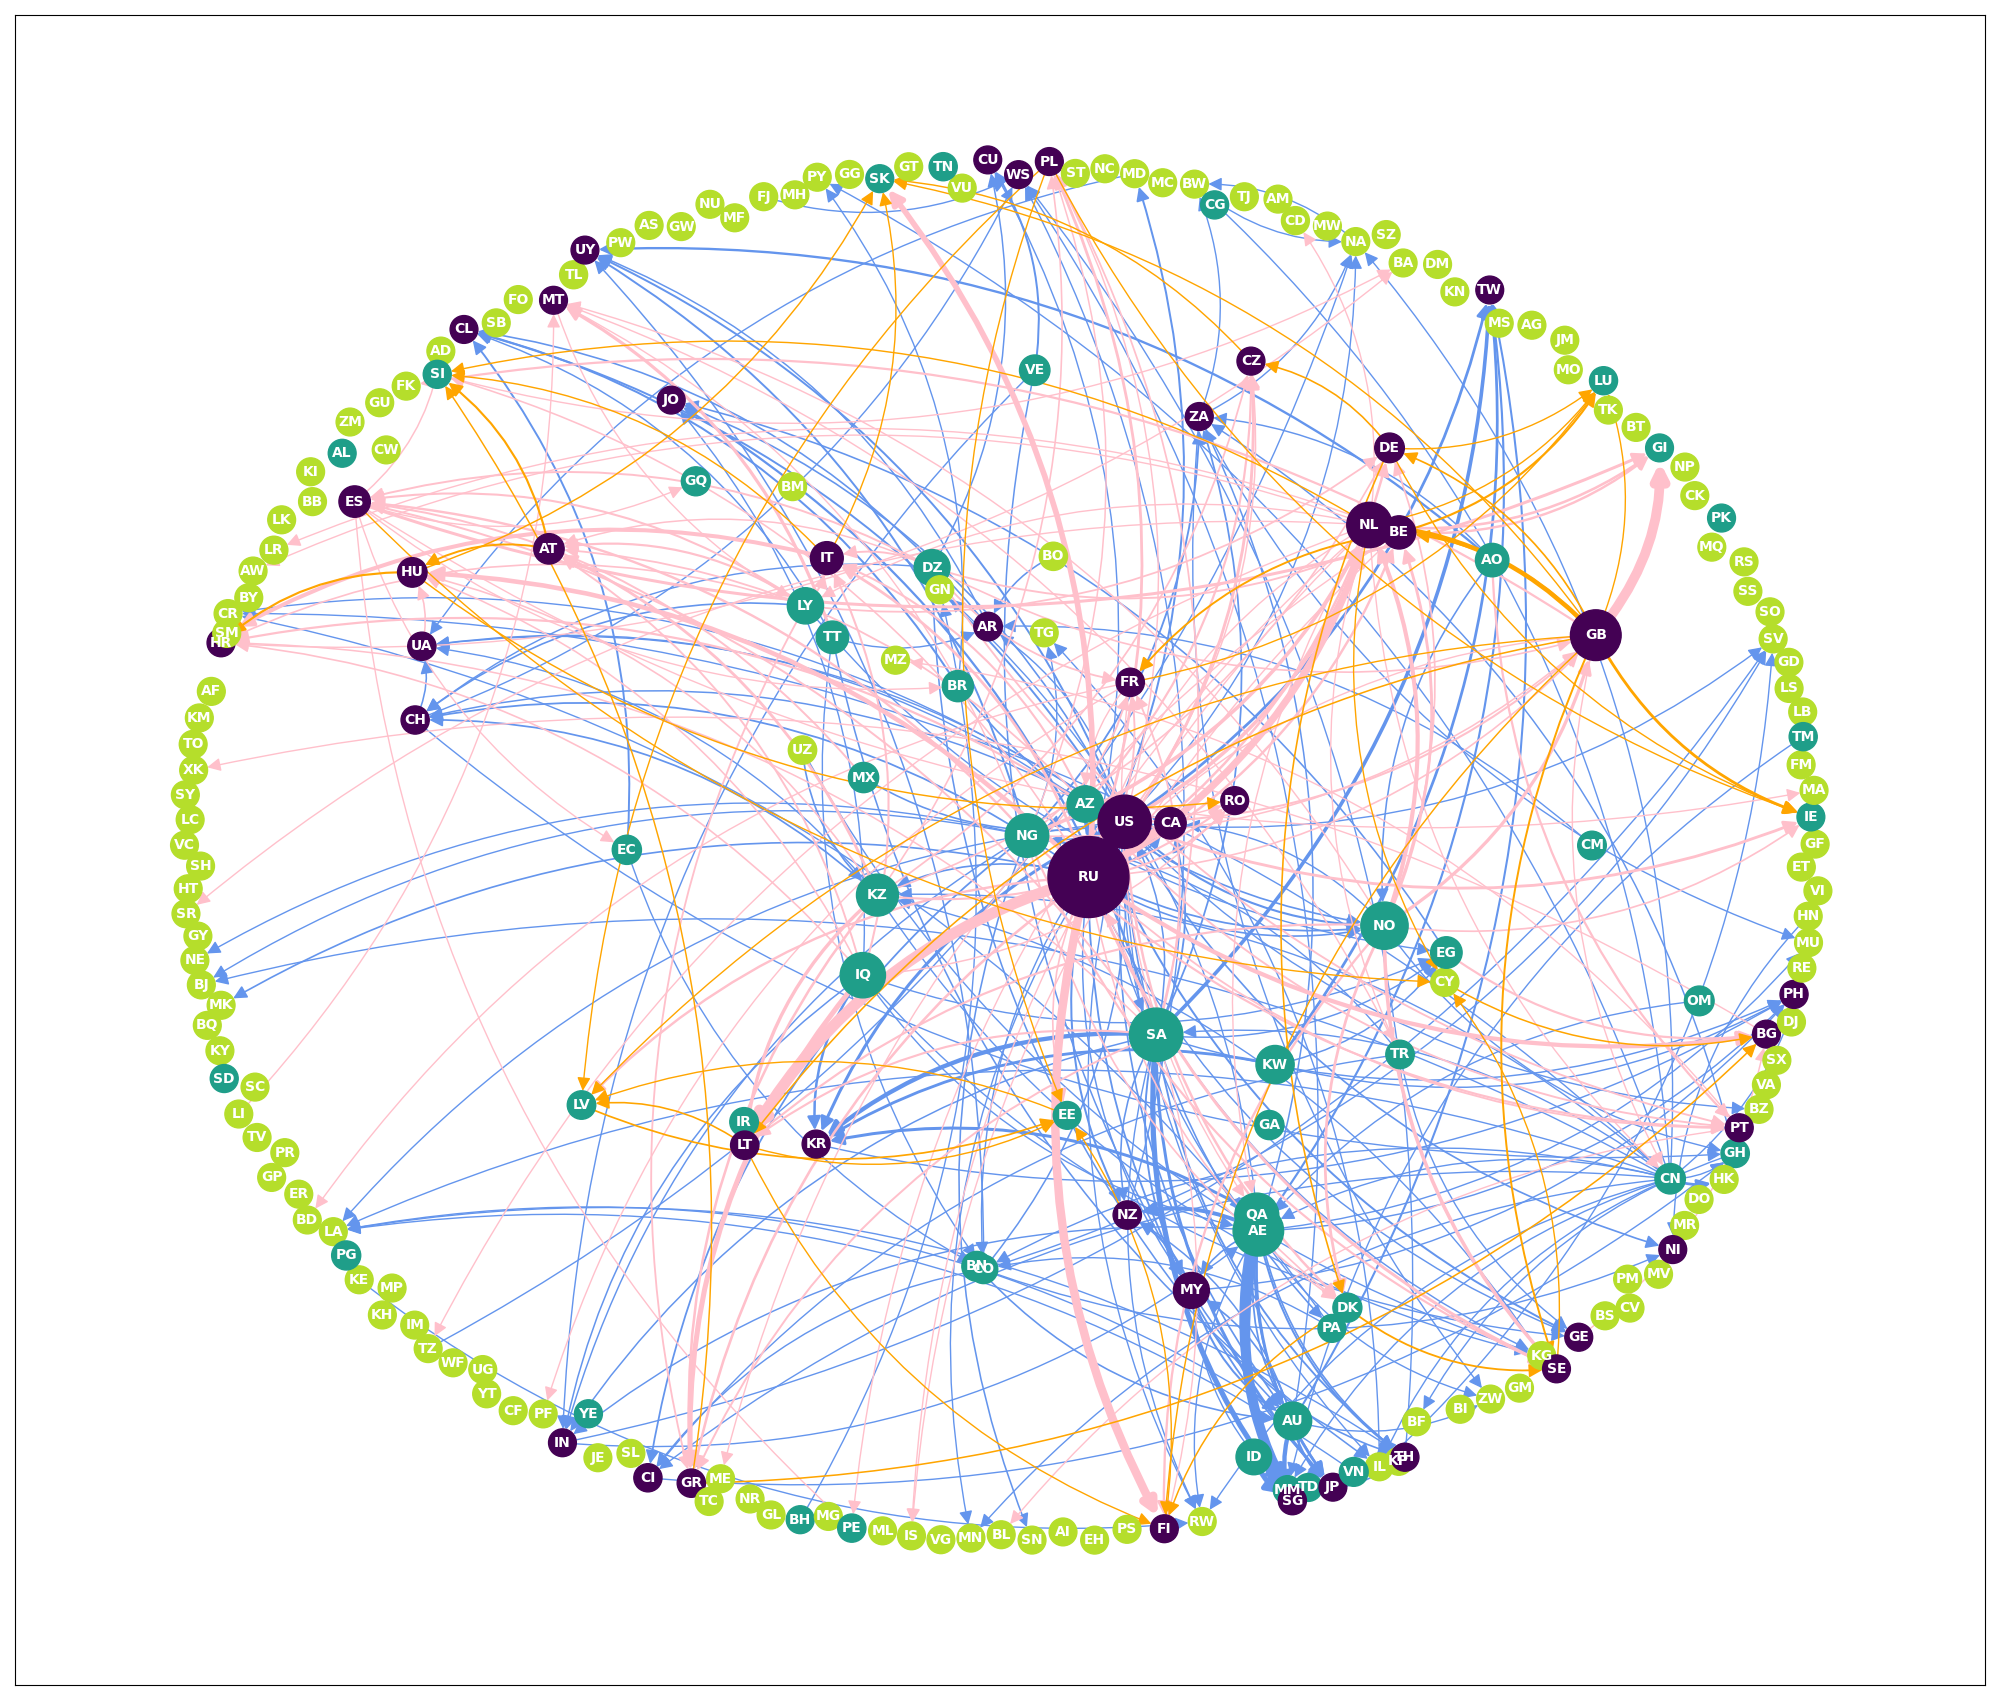
\includegraphics[width=\textwidth]{pics/full_y19_p06_force_146_dc.png}
        \caption{Degree Corrected SBM}
        \label{fig:gasnetworkdc}
    \end{subfigure}

    \begin{subfigure}{0.5\textheight}
        \centering
        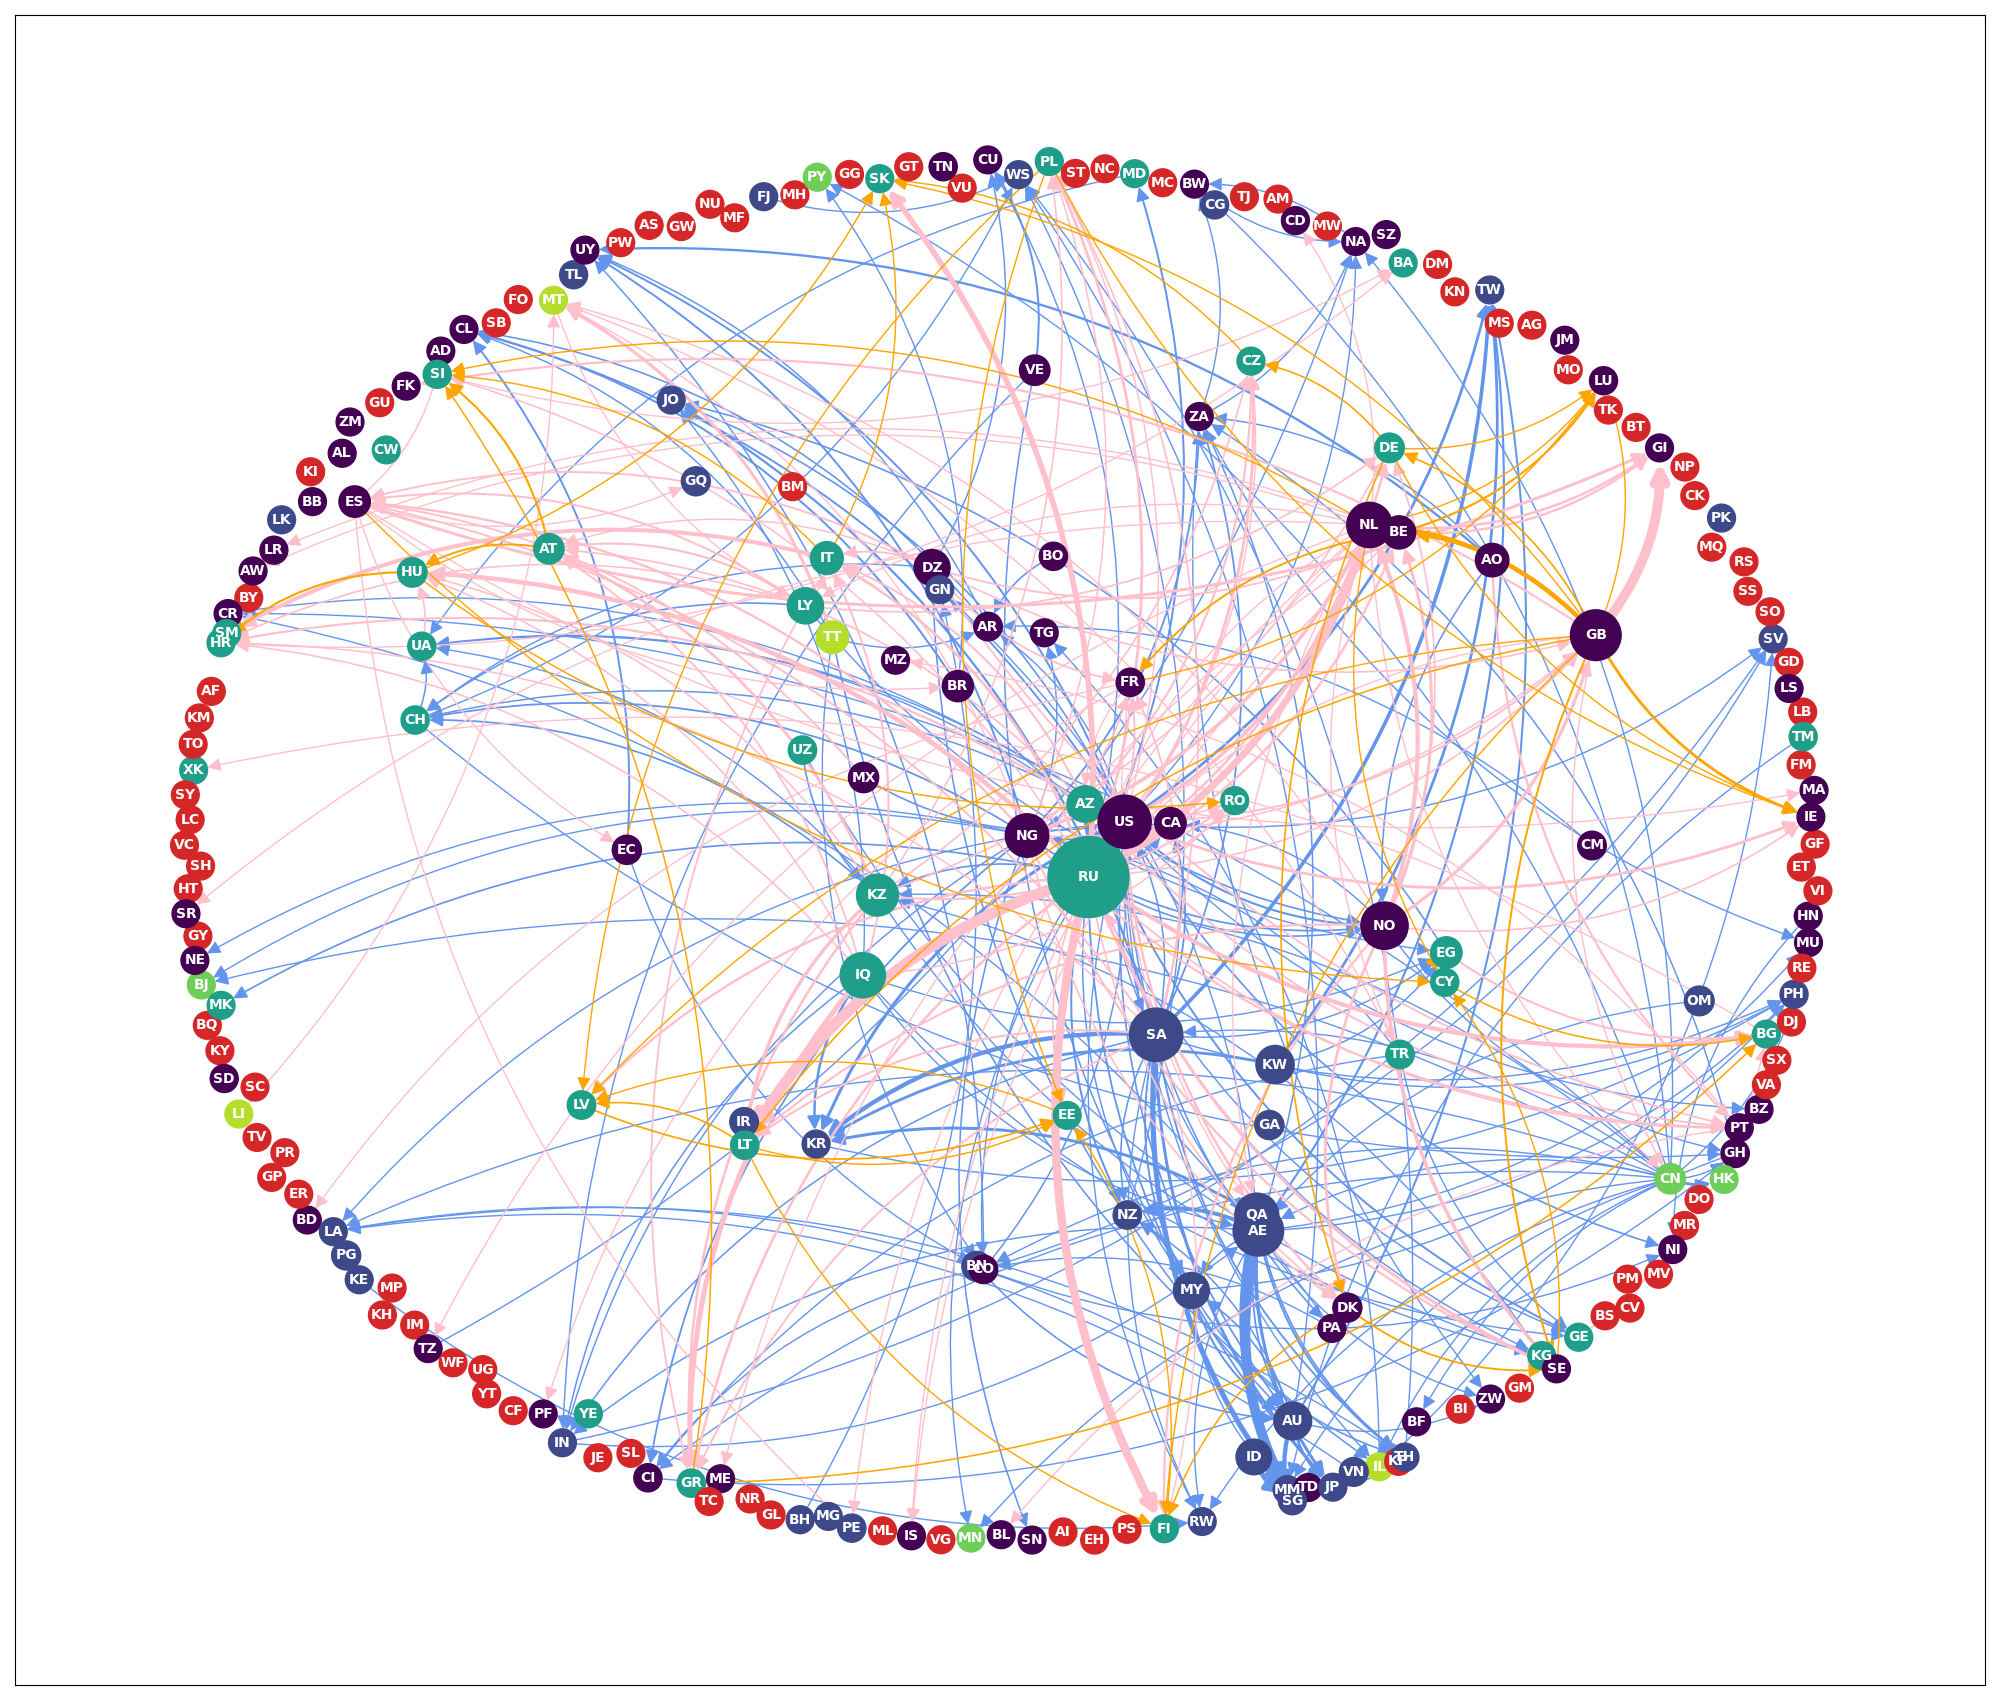
\includegraphics[width=\textwidth]{pics/full_y19_p06_force_147_lou.png}
        \caption{Louvain Method}
        \label{fig:gasnetworklou}
    \end{subfigure}
    \caption[Global trade network of \textit{Crude Petroleum and Natural Gas} in 2019, with communities.]{Global trade network of \textit{Crude Petroleum and Natural Gas} in 2019. The size of the node represents the \textit{out-strength} of that country. The color of the node corresponds to the block membership; the color of the edge is \textit{orange} for intra-EU exchanges, \textit{pink} for EU - non-EU exchanges and \textit{azure} for extra-EU exchanges. Only the top 10 import partnership for each country are shown.}
    \label{fig:gascommunities}
\end{figure}

